% @Author: AnthonyKenny98
% @Date:   2020-04-09 08:08:15
% @Last Modified by:   AnthonyKenny98
% @Last Modified time: 2020-04-09 08:33:23
For an $\epsilon \times \epsilon \times \epsilon$ grids, the grid space can be represented by an $\epsilon^3$ bit sequence.
A grid's index in the sequence is a function of its coordinates. This can be thought of as a 3 dimensional nested loop, incrementing most frequently on the $x$-axis, then the $y$-axis, then the $z$-axis. An index of 0 is the \gls{LSB} and an index of $\epsilon^3 - 1$ is the \gls{MSB}.

Mathematically, this can be thought of as the following: \\

$$f(x,y,z) = x + \epsilon y + \epsilon^2 z$$

In HoneyBee, this can computed efficienty by using shifts rather than multiplications, as long as $\epsilon$ is an even number. For $\epsilon=2$, SHAMT = 1. \\

$$f(x,y,z) = x + (y << \text{SHAMT}) + (z << \text{SHAMT} << \text{SHAMT}$$

Graphically, this can be represented as shown in Figure \ref{fig:honeybee_mapping} for $\epsilon = 2$.

\begin{figure}[H]
\begin{centering}
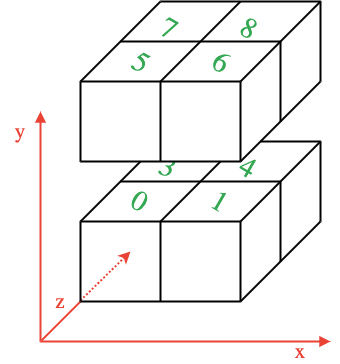
\includegraphics[width=0.6\linewidth]{appendices/honeybee/img/mapping.png}
\mycaption{Bit Sequence Mapping for a $2\times2\times2$ Grid Space}{}
\label{fig:honeybee_mapping}
\end{centering}
\end{figure}